\section{Einleitung}
\label{sec:03_01_einleitung}

Im Rahmen des Projekts \gls{sob} sollten Bundestagsprotokolle analysiert
werden, um den \enquote{Ton} des Bundestags zu bewerten. Das in diesem
Kapitel beschriebene Teilprojekt, das von Gruppe 2 bearbeitet wurde, hatte
die Wahl und Anwendung eines passenden Kommunikationsmodells zum Ziel. Zur
Erfüllung dieser Zielstellung wurde die \enquote{\gls{cme}}-Software erstellt.
Diese ist das letzte Pipeline-Element des Gesamtprojektes, das sich mit den Rohdaten der
Bundesregierung beschäftigt. Die in diesem Teilprojekt generierten Daten
stellen die Basis aller weiteren Verarbeitungsschritte dar.

\subsection{Zielstellung}
Die \gls{cme}-Software soll aus den \citetitle{OpenData2019}~\cite{OpenData2019}
\gls{xml}-Dateien der 19. Wahlperiode des Bundestages bzw. der leicht
abgewandelten Variante dieser Daten, welche von Gruppe 1 in Form von
\enquote{\gls{json}}-Dateien zur Verfügung gestellt werden, Interaktionen zwischen
Fraktionen und oder Abgeordneten extrahieren.

Für diese Extraktion werden die Rohdaten analysiert und darauf aufbauend ein
passendes Kommunikationsmodell gewählt. Um über neue Protokolle von Gruppe 1
informiert werden zu können, soll dafür eine Schnittstelle geschaffen werden.
Ebenfalls werden zur Weitergabe der Ergebnisse an die folgende Gruppe ein
Datenmodell, welches zur Speicherung der Ergebnisse dient, eine Schnittstelle
zur Weitergabe der Daten und eine weitere Schnittstelle, über welche Gruppe 3
bei neuen Daten benachrichtigt werden kann, entwickelt.

\subsection{Anforderungsdefinition}
\label{sec:03_requirements}

Auf Grundlage der im vorherigen Abschnitt beschriebenen Zielsetzung sowie der
Diskussionen in den Plenarsitzungen während des Semesters, erfolgt in diesem
Kapitel eine Zusammenfassung von funktionale Anforderungen, welche an das zu
entwickelnde System gestellt werden. Diese werden in Muss-, Soll- und
Kann-Kriterien unterteilt.

\begin{table}[H]
    \caption{Funktionale Anforderungen}
    \vspace{0.5cm}
    \renewcommand{\arraystretch}{2.5} % Default value: 1
    \centering
    \begin{tabularx}{\textwidth}{c|c|X}
        & \textbf{FR01} & \noindent\parbox[c]{\hsize}{
            Ein passendes Kommunikationsmodell und
            Datenmodell muss gewählt werden} \\
        & \textbf{FR02} & \noindent\parbox[c]{\hsize}{
            Das Ausgabeformat von Gruppe 1 muss eingelesen
            werden können} \\
        & \textbf{FR03} & \noindent\parbox[c]{\hsize}{
            Interaktionen basierend auf den Kommentaren
            zu Redebeiträgen müssen extrahiert werden} \\
        & \textbf{FR04} & \noindent\parbox[c]{\hsize}{
            Extrahierte Interaktionen müssen für den
            Zugriff späterer Gruppen persistiert werden} \\
        \textbf{Muss-Kriterien} & \textbf{FR05} & \noindent\parbox[c]{\hsize}{
            Spätere Gruppen müssen auf die persistierten
            Nachrichten zugreifen können} \\
        & \textbf{FR06} & \noindent\parbox[c]{\hsize}{
            Gruppe 1 muss die Möglichkeit haben, uns über
            die Verfügbarkeit neuer Daten zu
            benachrichtigen} \\
        & \textbf{FR07} & \noindent\parbox[c]{\hsize}{
            Gruppe 3 muss von uns benachrichtigt werden,
            wenn neue Daten zur Verfügung stehen} \\
        & \textbf{FR08} & \noindent\parbox[c]{\hsize}{
            Parteien und Abgeordnete müssen über Sitzungen
            hinweg eindeutig identifizierbar sein} \\
        & \textbf{FR09} & \noindent\parbox[c]{\hsize}{
            Daten von Gruppe 1 müssen aus deren MongoDB
            ausgelesen werden können} \\
        \hline

        \textbf{Soll-Kriterien} & \textbf{FR10} & \noindent\parbox[c]{\hsize}{
            Das Open Data Ausgabeformat des Bundestags soll
            eingelesen werden können} \\
        \hline

        \textbf{Kann-Kriterien} & \textbf{FR11} & \noindent\parbox[c]{\hsize}{
            Interaktionen innerhalb der Redebeiträge können
            extrahiert werden} \\

    \end{tabularx}
    \label{tab:03_requirements}
\end{table}

\subsection{Wahl des Kommunikationsmodells}
FR01 erfordert die Auswahl eines passenden Kommunikations- und Datenmodells.
Aus diesem Grund wurden zu Beginn des Semesters die bereits vorliegenden
Plenarprotokolle im \enquote{\citetitle{OpenData2019}}-Format der
Bundesregierung untersucht.

Bei dieser Untersuchung zeigte sich, dass die für uns interessanten Daten so
angeordnet sind, dass jede Sitzung in Tagesordnungspunkte unterteilt ist,
welche wiederum aus einer Vielzahl von Reden besteht. Eine solche Rede
enthält dabei Informationen über den Redner, die in einzelne Absätze
zerteilte Rede und optionale Kommentare anderer Parlamentarier oder
Fraktionen zu diesen Absätzen. So sind in diesen Strukturen Interaktionen
erkennbar, z.~B. in den Kommentaren an den Redner gerichtete Interaktionen oder
auch in den Absätzen Interaktionen zwischen dem Redner und anderen
Parlamentariern.

Basierend auf diesen Erkenntnissen und in Absprache mit Gruppe 3, 4 und 5,
welche für die Sentimentanalyse sowie die Auswertungen zwischen Fraktionen und
Abgeordneten verantwortlich sind, wurde ein Sender-Empfänger-Modell für die
Repräsentation der Interaktionen gewählt. In diesem kann der Sender und
Empfänger jeweils entweder ein Bundestagsabgeordneter oder eine Fraktion sein.
Auf Basis des Inhalts der Nachricht, die vom Sender zum Empfänger geschickt
wird, wird später von Gruppe 3 das Sentiment ermittelt.


\section{Umsetzung}\label{sec:03_02_umsetzung}
Auf Grundlage der definierten Anforderungen wurde im nächsten Schritt ein
Konzept für deren Umsetzung entwickelt. Dieses sowie die Umsetzung selbst
wird in den folgenden Abschnitten näher erläutert.

\subsection{\glsentryfull{cme}}
Für die Entwicklung der \gls{cme}-Software wurde die Programmiersprache Python
gewählt, da alle Teammitglieder bereits Kenntnisse in dieser mitbrachten und
um den folgenden Gruppen möglichst schnell erste Ergebnisse liefern zu können,
mit denen diese arbeiten können. So bietet Python eine Vielzahl an guten und
einfach zu nutzenden Bibliotheken, welche die Entwicklung einer solchen
prototypischen Applikation beschleunigen können. Z.~B. ist es innerhalb
weniger Zeilen möglich, einen funktionsfähigen \gls{rest}-Endpoint zur
Verfügung zu stellen.

Aus den funktionalen Anforderungen FR05, FR06 und FR07 ergibt sich, dass eine
Kommunikation zu den Gruppen 1 und 3 nötig ist. Aufgrund hoher Kompatibilität
wurde sich für eine \gls{rest}-Schnittstelle entschieden. Diese \gls{api} wurde in dem
Python-Modul \enquote{api.py} mithilfe der FastAPI-Bibliothek implementiert. Sie
beantwortet Anfragen zu Protokollen (Sessions), Fraktionen (Factions) und
\glspl{mdb}. Außerdem wird eine SWAGGER-Dokumentation
bereitgestellt.

Zur Steuerung der Anwendung wird ein \gls{cli}, welches im \enquote{cli.py}-Modul umgesetzt
wurde, in Form der \gls{cme}-Applikation zur Verfügung gestellt. Dieses ist in
verschiedene Unterkommandos aufgeteilt. Mithilfe dieser ist es z.B. möglich
Protokolle manuell aus dem lokalen Speicher einzulesen (\gls{xml}- oder \gls{json}-Format)
oder den Server zu starten. Mit \enquote{init} werden erstmalig Bundestagsabgeordnete
eingelesen. \enquote{dump} ermöglicht die Interaktion mit der Datenbank, um einzelne
Dokumente daraus zu extrahieren.

Um die Anwendungslogik von der Business-Logik zu trennen, wird der \enquote{Controller}
eingeführt. Es ist das zentrale Modul, welches die Prozesse koordiniert.

Für die generische Verarbeitung der Rohdaten in den verschiedenen Datenformaten
von Gruppe 1 (FR02) und der Open Data Protokolle des Bundestags (FR10) wurde
das \enquote{Data}-Modul implementiert. Dieses wandelt die Rohdaten unter anderem in
sogenannte InteractionCandidates um, welche dann mithilfe des \enquote{Extraction}-
Moduls verarbeitet und ausgewertet werden (FR03 und FR11). So extrahiert dieses
aus den InteractionCandidates die stattgefundenen Interaktionen basierend auf
dem Sender-Empfänger-Modell und legt diese in einem sogenannten Transcript ab.
Dieses Transcript wird anschließend mithilfe des \enquote{Database}-Moduls, welches für
jeglichen Datenbankzugriff zuständig ist, in der Datenbank abgelegt.

Zuletzt enthält \enquote{Domain} Datenmodelle für verschiedene Objekte, wie z.~B. \gls{mdb},
Faction \& Interaction. Es wird von so gut wie jedem Modul benutzt.

Die soeben beschriebenen Module und der damit verbundene Kontrollfluss zwischen
diesen ist in \autoref{fig:03_project_structure} dargestellt.

\begin{figure}[ht]
    \begin{center}
        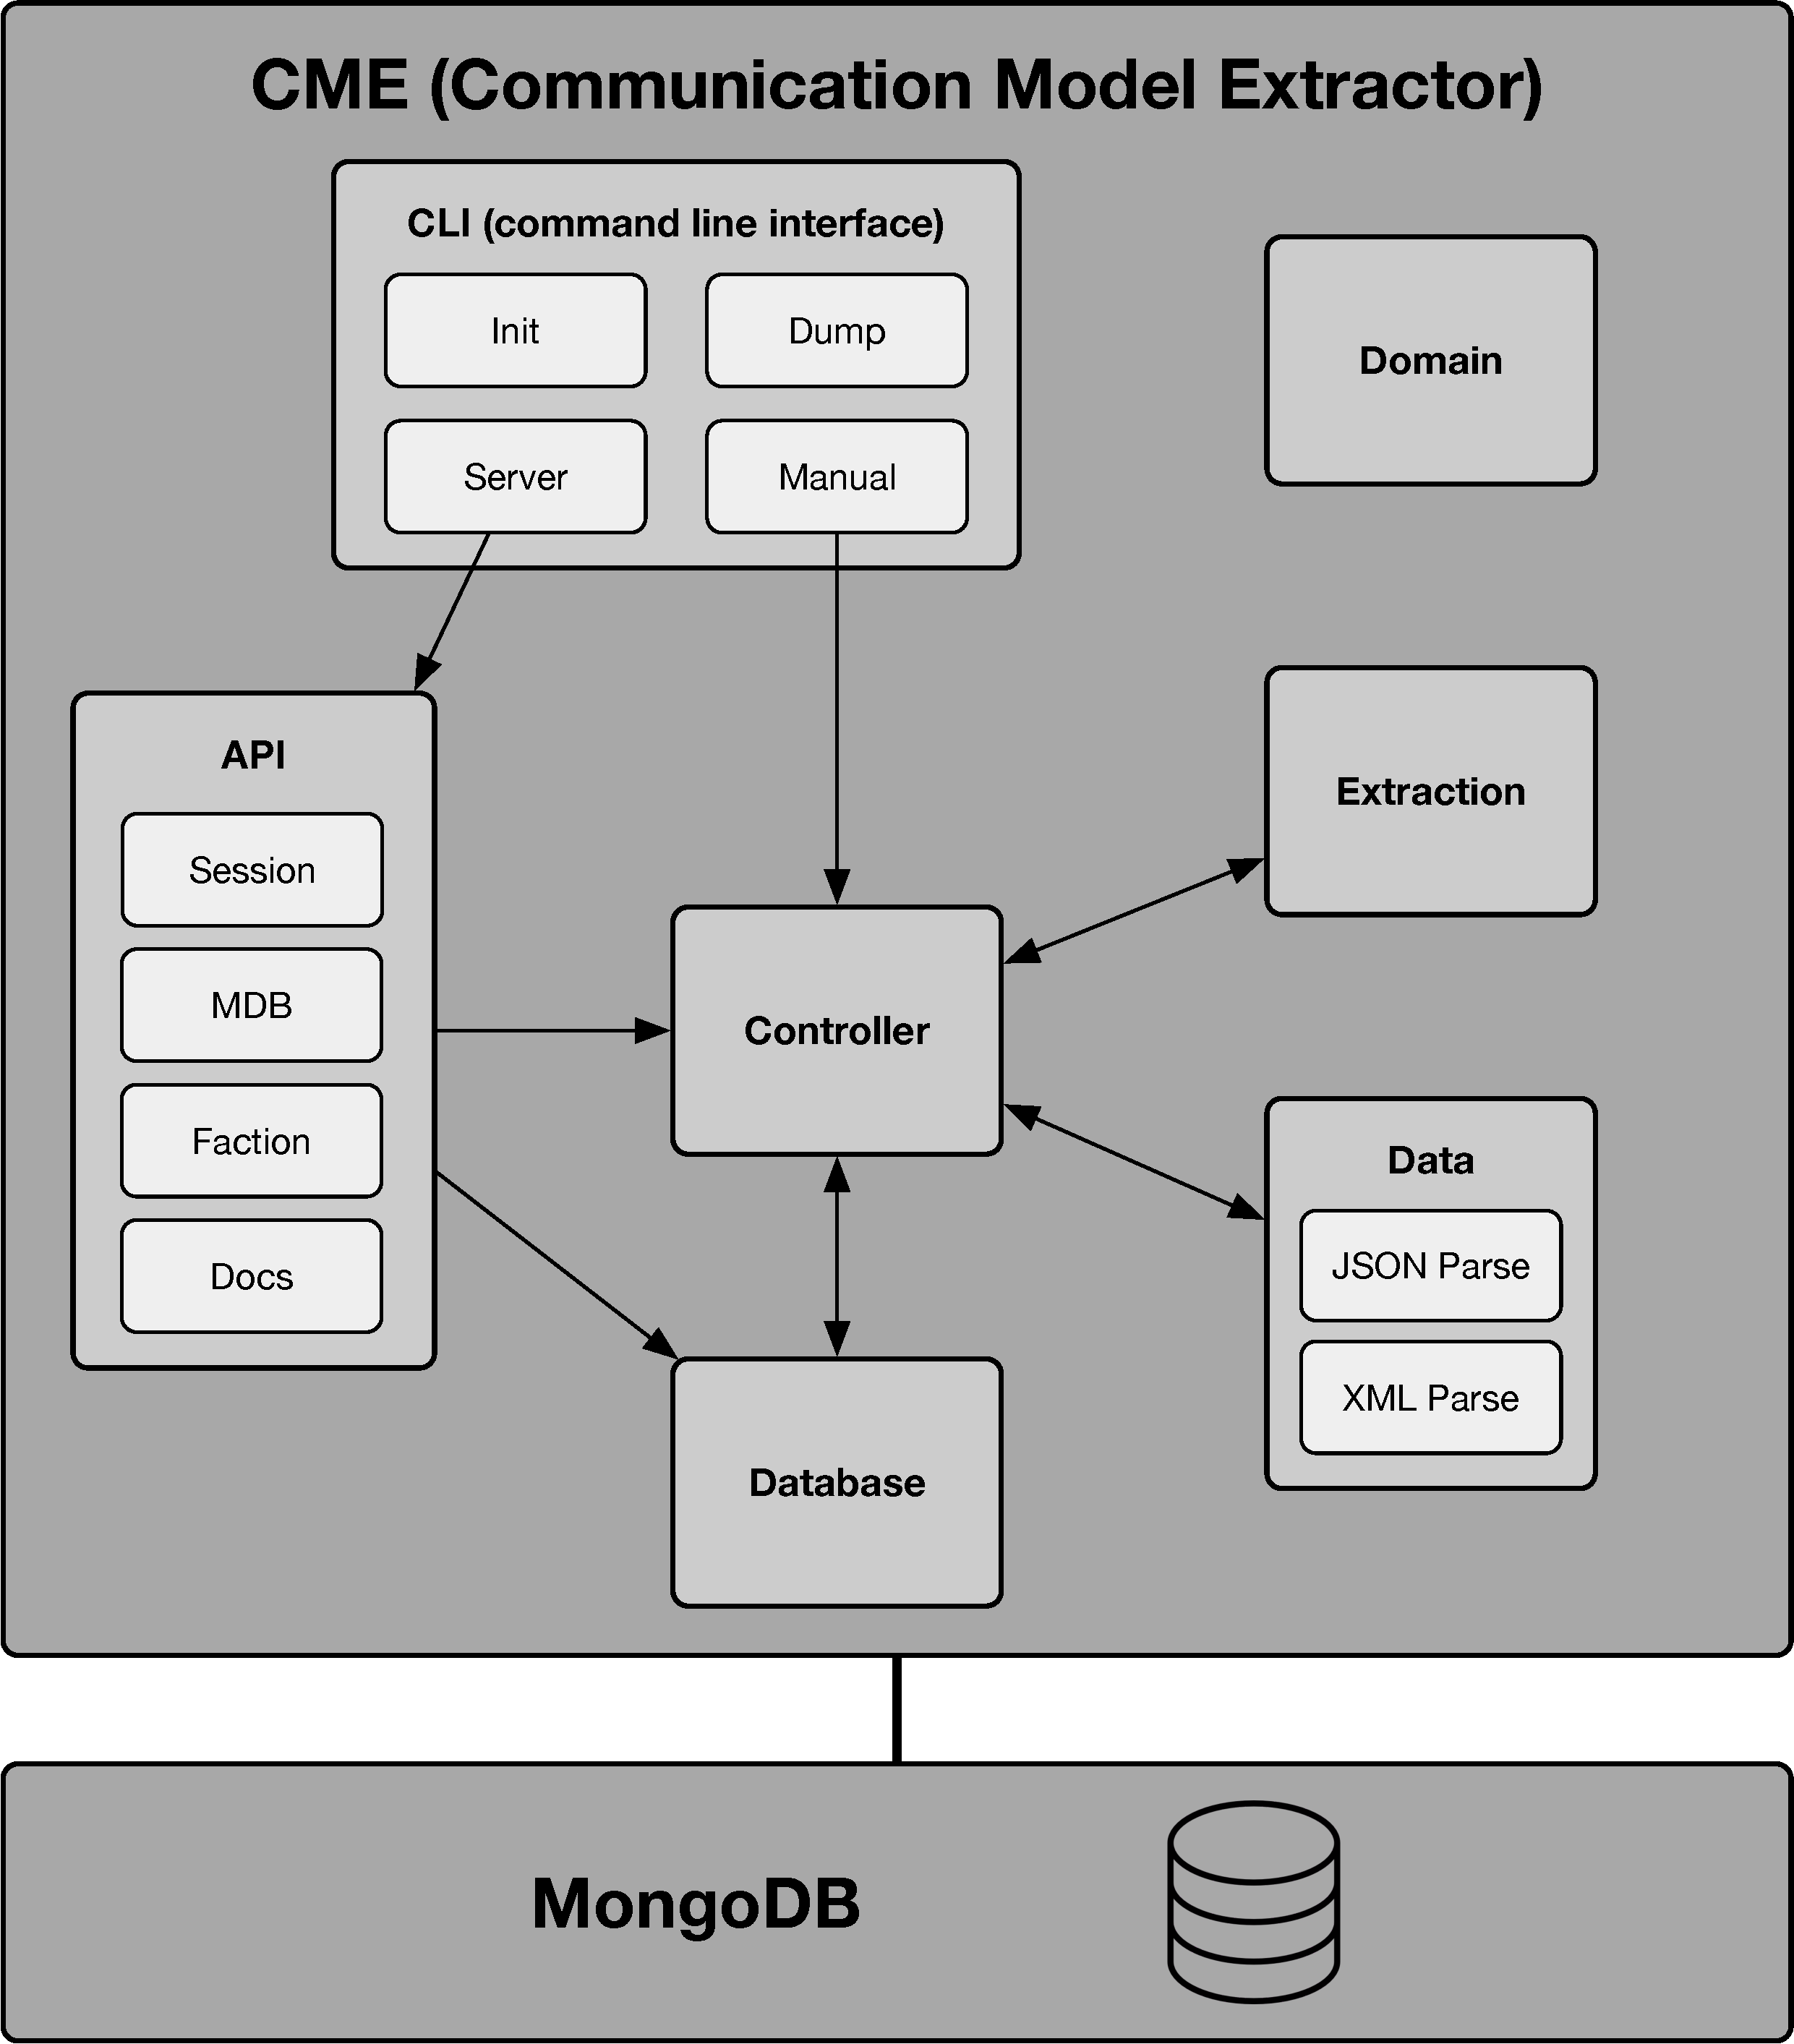
\includegraphics[width=0.6\textwidth]{images/03-cme/Project-Modules.pdf}
    \end{center}
    \caption{Applikations-Architektur}
    \label{fig:03_project_structure}
\end{figure}

\subsection{Eingabeformate}
Wie in den Anforderungen FR02 und FR10 definiert, muss als Eingabeformat
einerseits das \gls{json}-Format der Gruppe 1 und andererseits soll auch das
Open Data \gls{xml}-Format des Bundestags unterstützt werden. So wurden
spezielle Parser für die jeweiligen Formate entwickelt, deren Ausgabe gleich
formatiert ist und somit für die nächste Instanz eine einheitliche
Schnittstelle bildet. Dieses Ausgabeformat enthält dabei neben Metadaten zur
Sitzung selbst, wie z.~B. den Sitzungsstartzeitpunkt oder die Sitzungsnummer,
sogenannte InteractionCandidates. Diese gruppieren, wie der Name bereits
nahelegt, Daten, welche eventuelle, für die Auswertung relevante, Interaktionen
enthalten. So gruppiert ein InteractionCandidate den Redner (Speaker),
einen Absatz von dessen Rede (Paragraph) und den eventuell darauf folgenden
Kommentarblock (Comment).

\subsection{Methodik der Kommunikations-Analyse}
Die zu analysierenden Daten (InteractionCandidates) bieten zwei verschiedene
Kommunikationstypen als Datengrundlage für die Erkennung von Interaktion:

\begin{enumerate}
    \item \textbf{Kommentare (FR03)}: werden von den Redeteilen gesondert
    dargestellt und mit zusätzlicher Information bezüglich der
    kommunikativen Einordnung des Beitrags versehen.
    \item \textbf{Redeteile (FR10)}: werden in den Protokollen als
    Paragraphen oder sinngemäß als Absätze aufgeführt.
\end{enumerate}

Aufgrund der Unterschiedlichkeit mussten beide Typen gesondert analysiert werden.

\subsubsection{Kommentare}

Kommentare werden nach rigiden strukturellen Regeln in den Protokollen der
Bundestagssitzungen erfasst und liefern unter anderem Informationen zum
Sender des Kommentars. Dieser kann eine oder mehrere Fraktionen oder eine
oder mehrere an der Sitzung teilnehmende Personen sein. Kommentare lassen sich
in die Folgenden drei Kategorien unterteilen:

\begin{itemize}
    \item \textbf{Publikumsresonanzen}: Z.~B. Beifall oder Entrüstung des
    Senders, bei der eine genaue Zitierung durch die Stenographen nicht
    möglich ist. Hier folgen Sender durch Präpositionen abgetrennt auf
    den Kommentarinhalt. Bsp.: \enquote{Beifall bei der CDU};
    \enquote{Zurufe von der Linken und Grünen}

    \item \textbf{Zitate}: Hier wird der Wortlaut eines Kommentars
    wiedergegeben. Bei diesen Kommentaren wird die kommentierende Person
    dem Wortlaut vorangestellt und durch einen Doppelpunkt abgetrennt.
    Bsp.: \enquote{Dr. Klaus Hermann: Ganz toll gemacht}; \enquote{Dr.
    Alexander Gauland: Schwachsinn}

    \item \textbf{Beobachtungen der Protokollanten}: Spezielle Situationen in
    denen ein oder mehrere Sitzungsteilnehmer nennenswerte Handlungen
    vornehmen. Auch hier wird in der Regel der Sender der Nachricht
    vorangestellt, wenngleich keine Trennung durch einen Doppelpunkt
    erfolgt. Bsp.: \enquote{Manfred von Kuchenhausen verlässt die Sitzung}

\end{itemize}

Je nach erkannter Kommentarform kommen also verschiedene strukturelle
Analyse-Vorgänge für die Feststellung von Sendern zum Einsatz.

\paragraph{Kommentare mit abweichender Struktur}

Es gibt weitere Eigenschaften, die die Extraktion der Interaktionen
erschweren. So können pro Kommentar-Abschnitt mehrere Strukturen mit
unterschiedlichen Inhalten auftreten, oder es werden insbesondere bei
Publikumsresonanzen mehrere Absender aufgeführt (etwa
\enquote{Beifall von SPD und die Linke}), wodurch zusätzlich eine korrekte
Auftrennung der Sender auf Basis von Konjunktionen bzw. Interpunktion
notwendig wird. Außerdem gibt es gelegentlich sekundäre Kommentare, bei denen
auf vorherige Kommentare reagiert wird. Die einzigen zuverlässigen
Formatierungen, die auf solche Verhältnisse hinweisen, sind die expliziten
grammatikalischen Strukturen nach der Namensnennung:
\enquote{an [neuer Empfänger] gerichtet} bzw. \enquote{zur [Ziel-Fraktion] gewandt}
wirken innerhalb von Kommentaren als klares Merkmal für einen vom Redner
abweichenden Empfänger. Das Schlüsselwort \enquote{Gegenruf} wird darüber
hinaus häufig verwendet, um auf einen Dialog zwischen Kommentierenden
hinzuweisen - da in diesen Fällen allerdings der Kommentarinhalt oft
mindestens teilweise weiterhin auf den Redner abzielt, wurde bei solchen
Kommentaren ebenfalls der Redner als Empfänger verwendet. Diese
Problematik könnte in Fortsetzungen der Arbeit eventuell präziser behandelt
werden, da in längeren Kommentar-Dialogstrukturen recht häufig auf die
eindeutige Empfängerbezeichnung verzichtet wird. Dadurch werden in unserer
Methode viele für menschliche Leser offensichtliche Interaktionen nicht als
solche registriert. Nicht zuletzt werden die genannten syntaktischen
Strukturen gelegentlich durch Rechtschreib- oder Zeichensetzungsfehler
durchbrochen, wobei in diesen Fällen die gesamte Interaktion verloren geht.

\subsubsection{Redeteile}
Redeteile besitzen weniger Struktur als Kommentare, da sie nicht den Regeln der
Stenographen unterliegen, sondern des individuellen Redners. So muss der
Empfänger einer Aussage erst ermittelt werden. Redeteile wurden daher auch nur
als Interaktionen gewertet, sobald Fraktionen oder Mitglieder des Bundestags
als mögliche Interaktionsempfänger im Fließtext erkannt wurden.

Die Erkennung von \glspl{mdb} erfolgt über die Feststellung bekannter, eindeutiger
Nachnamen, denen eine formale Anrede (Herr/Hr., Frau/Fr., Kollege, Doktor)
vorangeht. Parteien wurden anhand von ihren Namen bzw. deren Abkürzungen,
beziehungsweise durch gängige aber eindeutige Kurzformen identifiziert. Die
festgestellte Person oder Partei wurde anschließend als Empfänger der Nachricht
behandelt, während die sprechende Person, also der durch den
Sitzungspräsidenten zuletzt eingeleitete Redner, die Rolle des Absenders
einnahm.

Die Empfängerermittlung bei Redeanteilen verblieb in der entstandenen
Implementierung in einem recht rudimentären Zustand, da viele der inhärenten
Probleme des Ansatzes nicht behandelt werden konnten. So hat etwa die
Unterscheidung zwischen mehreren \glspl{mdb} mit gleichen Nachnamen oder die
kolloquiale Verwendung von Farben (\enquote{Rot} für SPD oder die Linke) oder
Begriffen (\enquote{Liberale} stellvertretend für die FDP) als Substitut für
Fraktionen zur Generierung vieler falscher Interaktionen geführt. So kann
z.~B. \enquote{Rot} einerseits in Kontexten wie \enquote{roter Gentechnik} und
andererseits zur Nennung der SPD genutzt werden. Aus diesem Grund wurde die
Funktionalität wieder entfernt. Daher werden nur solche Interaktionen gewertet,
welche sich an eindeutig identifizierbare \glspl{mdb} oder Fraktionen richten.
Nachnamen wie \enquote{Müller}, die mehrere \glspl{mdb} bezeichnen können, aber
auch in anderen Sachverhalten eingesetzte Begriffe, wie \enquote{Union}, wurden
somit aus der Schlüsselwort-Liste entfernt, mit der die Redeabschnitte
abgetastet wurden. Es sollte allerdings nicht außer Acht gelassen werden, dass
Interaktionen in Redeteilen nach unseren Messungen einen recht geringen Anteil
der Interaktionen im Bundestag ausmachen. Die Steigerung der Anzahl erkannter
Interaktionen durch unsere Methode der Redebeitrag-Analyse betrug für die
bisherigen Protokolle der 19. Wahlperiode lediglich 8\% gegenüber der
alleinigen Betrachtung der Kommentare, was dafür spricht, dass auch nach
Aufnahme von weiteren Fraktionsbegriffen bzw. Nachnamen in die Betrachtung nur
relativ wenige Interaktionen hinzukommen würden.

\subsection{Ermittlung von teilnehmenden Personen}
Personen müssen über Sitzungen hinweg eindeutig identifizierbar sein, damit
nachfolgende Gruppen Informationen zu Parteizugehörigkeit und Namen korrekt
zuweisen können (FR08). Personen werden in der \enquote{mdb}-Collection der MongoDB
gesammelt. Initialisiert werden kann diese Liste mithilfe der Stammdaten der
Bundestagsabgeordneten des Bundestags. Diese, als \gls{xml} zur Verfügung gestellte,
Liste enthält alle relevanten Informationen, die bei der Identifizierung
helfen (Namen und Namensänderungen, Parteizugehörigkeit mit von-bis-Datumsangabe,
Titel etc.).

Da die Stammdaten unvollständig sind, auch weil Gastredner Reden halten oder
Bundestagsabgeordnete in den Stammdaten fehlen, müssen weitere Redner während
der Analyse hinzugefügt werden. Gerade in den Kommentaren können meist Vor-
und Nachnamen extrahiert werden, um ein Abgleich mit den \gls{mdb}-Daten
vorzunehmen. Leider werden Namen oft inkonsistent geschrieben (z.~B. wird
der zweite Vorname manchmal ausgeschrieben, abgekürzt oder weggelassen) oder
die Stenographen vertippen sich. Auch wird das Format der Kommentarsektion
nicht immer eingehalten.

Weil fehlende Redner und Rechtschreibfehler nicht unterschieden werden können,
gelangen doppelte Einträge in die Datenbank. Es wurden Mechanismen eingebaut,
um solche Fehler zu erkennen. Diese können jedoch nicht ganz ausgeschlossen werden.

\subsection{Infrastruktur-Setup mit Docker}
Um ein einfaches Deployment zu ermöglichen, wurde ein Container-basierter
Deploymentansatz gewählt. Dieser nutzt sowohl einen Container für die im
Rahmen des Teilprojektes erstellte Software, als auch für die MongoDB, welche
für die Persistierung der Daten genutzt wird.

Die beiden Container werden mithilfe von docker-compose verwaltet und
konfiguriert. Dabei gibt es neben der docker-compose-Konfiguration für das
Deployment auch eine zweite für die lokale Entwicklung. Diese enthält primär
die MongoDB, da während der Entwicklung der lokale Code mit den entsprechenden
Modifikationen genutzt werden soll und z.~B. ein ständiges Neubauen des
Applikation-Images und damit unnötiger Zeitaufwand verhindert werden soll.

Die Konfiguration des MongoDB-Containers erfolgt über Environment-Variablen
und ein \textit{mongo-init.sh}-Skript, welches beim ersten Starten des
Containers von dem MongoDB-Server ausgeführt wird. Dieses legt basierend auf
Environment-Variablen einen neuen DB-User (cme) an, welcher nur in einer
Datenbank mit dem Namen \textit{cme\_data} Lese- und Schreibrechte hat.

Das Applikation-Image wird bei jedem Starten der docker-compose-Umgebung
frisch gebaut und enthält die \gls{cme}-Software, welche durch die Tatsache,
dass es sich dabei um ein installierbares Python-Package handelt, einfach nur
dort installiert werden muss.

Zusätzlich wurde die Deployment-docker-compose-Konfiguration so konfiguriert,
dass ein Zugriff auf die Container von außen nicht möglich ist. Dies bedeutet
einerseits, dass der DB-Port des MongoDB-Containers nur durch den
\gls{cme}-Container erreichbar ist und andererseits, dass die
\gls{rest}-Endpoints des \gls{cme}-Containers nur über eine Verbindung von
Localhost aus erreichbar sind. Der Zugriff von außen erfolgt über einen
zusätzlich konfigurierten nginx-Reverse-Proxy. Dieser hat neben \gls{ssh} den
einzigen nach außen hin geöffneten Port auf dem Server. Somit muss jeder
Request durch diesen Reverse-Proxy fließen, bevor er in die
docker-compose-Umgebung gelangt.

\subsubsection{Datensicherheitsvorfall}

Während der initialen Konfiguration der Infrastruktur wurde der interne
Kommunikationsport des genutzten MongoDB-Containers aufgrund einer
fehlerhaften docker-compose-Konfiguration durch den Docker-Daemon nach außen
geöffnet und nicht, wie gedacht, nur lokal. So konnte auf die so für den Rest
des Internets frei zugängliche MongoDB von außen zugegriffen werden und diese
wurde kompromittiert.

Nachdem diese Situation dem Team bekannt wurde, wurde dies den entsprechenden
Parteien gemeldet und das System wurde ein zweites Mal aufgesetzt. Für diese
zweite Konfiguration wurde ausgiebig die vorliegende
docker-compose-Konfiguration überprüft. Dabei stellten wir fest, dass die
Verwendung des \textit{ports}-Arguments ohne die Angabe einer expliziten \gls{ip},
wie es in vielen docker-compose-Tutorials zu finden ist, dazu führt, dass der
Docker-Daemon diesen Port mithilfe einer zusätzlichen \gls{ip}-Tables-Chain nach
außen hin öffnet. Aus diesem Grund wurde in der offiziellen Dokumentation als
Lösung nach alternativen Möglichkeiten gesucht, Ports freizugeben. Dort wurde
einerseits die bereits erwähnte Lösung gefunden, welche durch die explizite
Angabe einer \enquote{Bind}-\gls{ip}-Adresse wie z.~B. hier
\enquote{127.0.0.1:9001:9001} dazu führt, dass nur Anfragen, die über diese
Adresse erfolgen, beantwortet werden. Andererseits wurde das
\textit{expose}-Argument entdeckt, welches diesen Port nur für alle
Docker-Container innerhalb derselben docker-compose-Umgebung freigibt.

Zur vollständigen Beseitigung des Problems wurde schließlich, wie auch schon
im vorherigen Abschnitt beschrieben, das \textit{expose}-Argument genutzt,
um den MongoDB-Container nur innerhalb der docker-compose-Umgebung zugänglich
zu machen. Zusätzlich wurde das Portbinding des \gls{cme}-Containers, welcher
den \gls{rest}-Service enthält, auf Localhost beschränkt. Die eigentliche
Auflösung von außen erfolgt dann über einen nginx-Reverse-Proxy, welcher im
Hostsystem unter einem nicht privilegierten Nutzer läuft. So ist jeglicher
Zugriff auf die docker-compose-Umgebung von außen nicht mehr möglich und muss
durch den Reverse-Proxy.

\subsection{Schnittstelle für Zugriff auf den Communication Model Extractor}

Um den gewünschten Workflow einer Pipeline zu ermöglichen, entschieden wir
uns eine \gls{api} anzubieten, wodurch die Kommunikation zur vorherigen und
folgenden Gruppe realisiert wurde.

\begin{figure}[ht]
    \begin{center}
        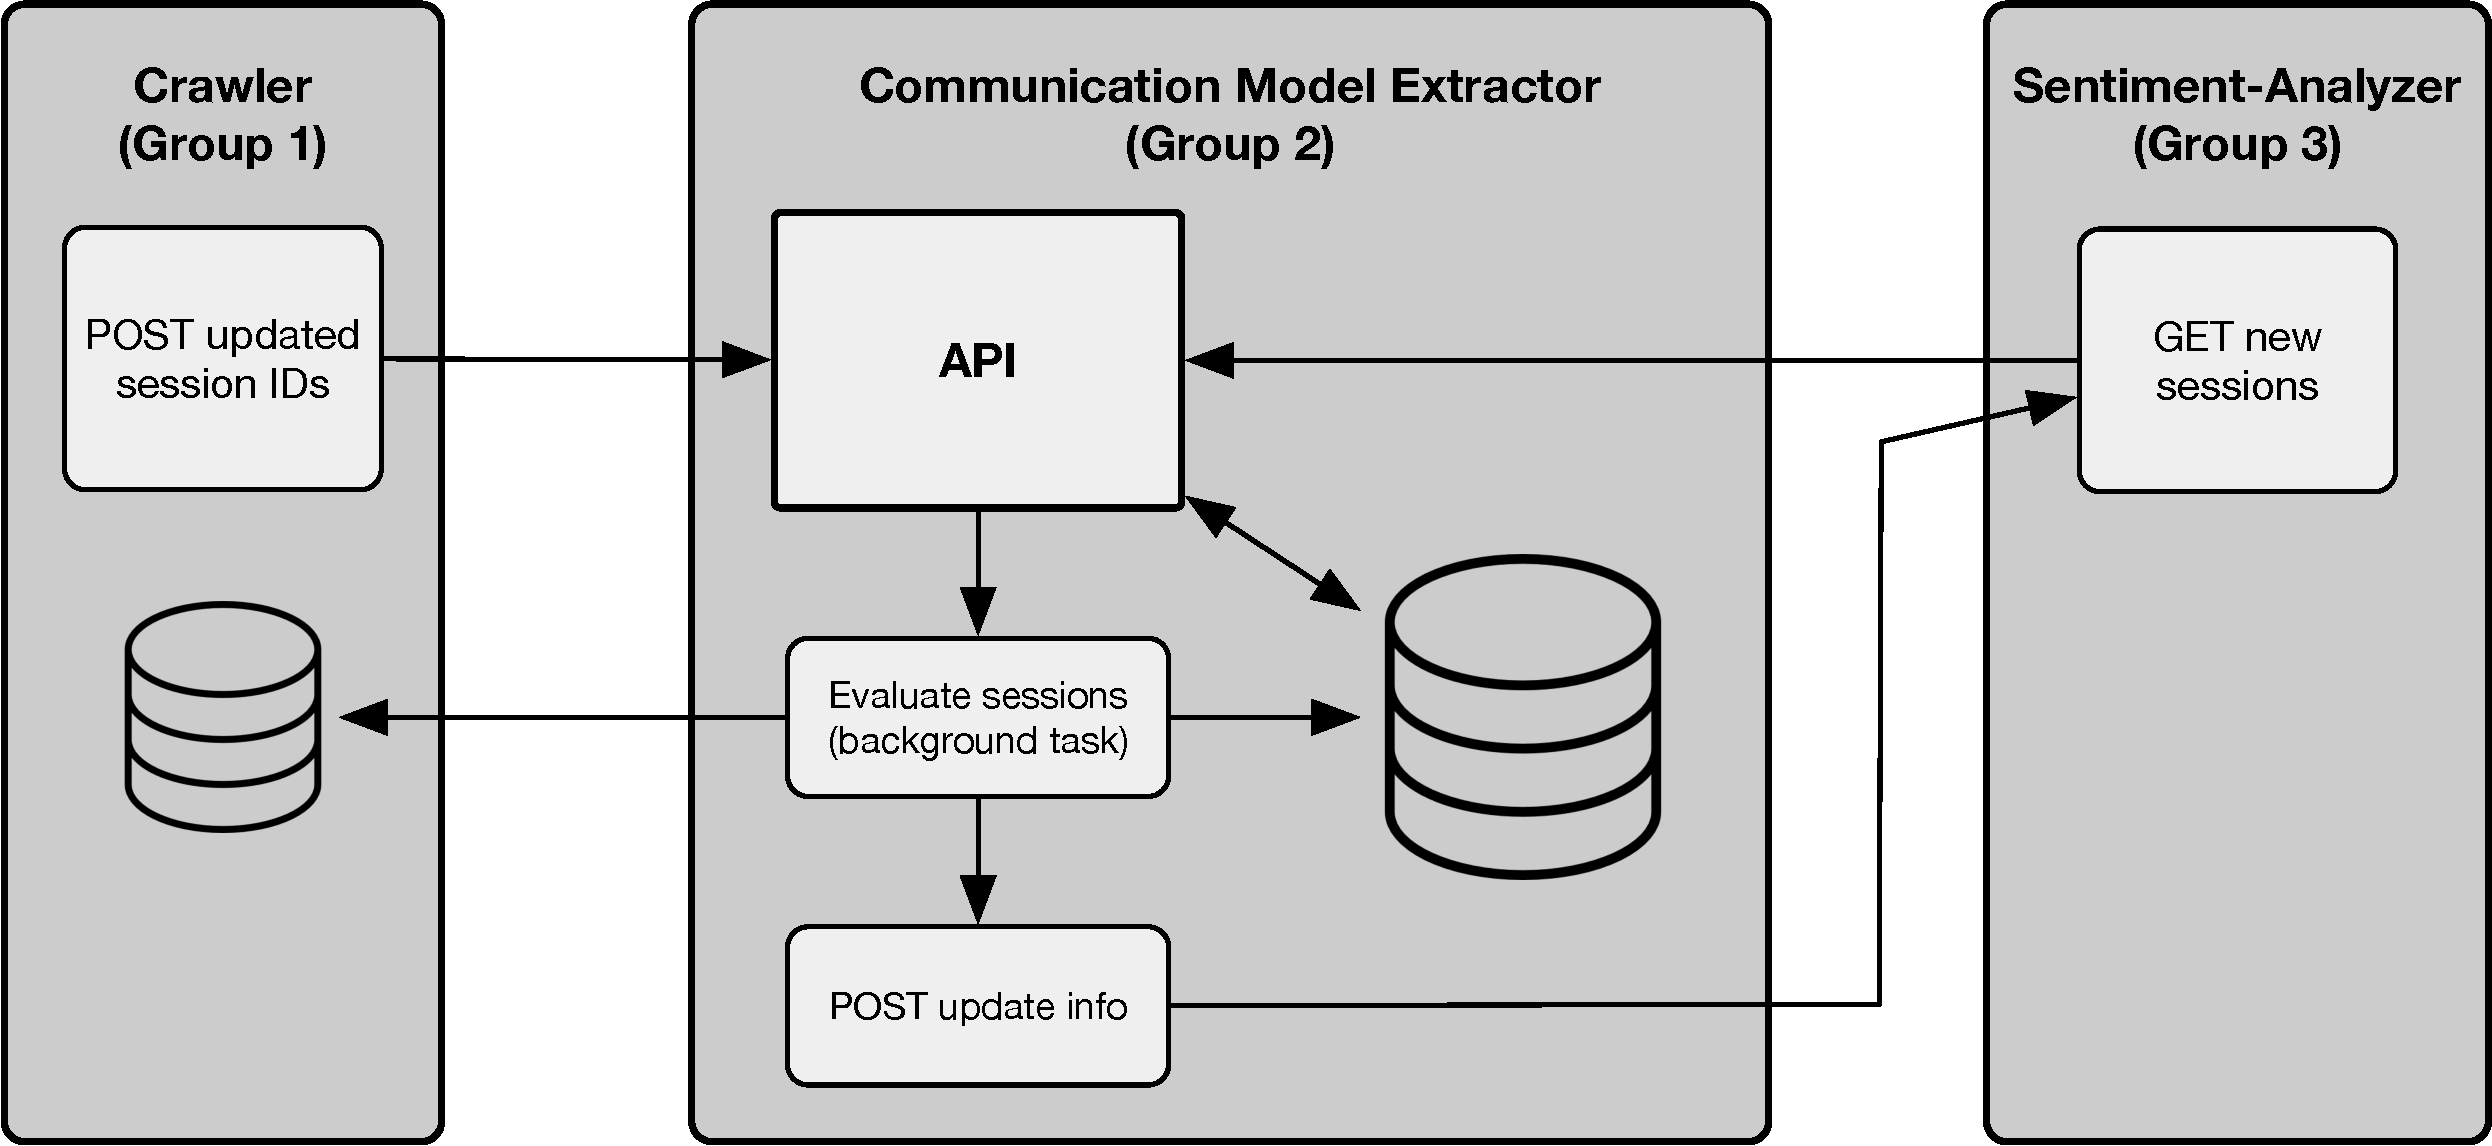
\includegraphics[width=\textwidth]{images/03-cme/Communications.pdf}
    \end{center}
    \caption{\gls{api}-Kommunikationsfluss}
    \label{fig:03_api_call_flow}
\end{figure}

Es wurde sich mit Gruppe 1 darauf geeinigt, dass der \gls{cme} einen Endpunkt
anbietet, um die Information zu erhalten, wenn neue Protokolle aus dem
Bundestag in deren Datenbank kreiert wurden. Nach dem Erhalt der Zugangsdaten konnte
auf die Datenbank der Gruppe 1 zugegriffen werden können. So werden die
Protokoll-ID's an \url{http://infosys2.f4.htw-berlin.de:9001/cme/data/} gesendet
und der \gls{cme} holt sich die gewünschten Protokolle zu einem späteren Zeitpunkt
aus deren Datenbank. Danach kann die Auswertung geschehen.

Um der darauffolgenden Gruppe Bescheid zu geben, wird nach dem Prozess der
Auswertung ebenfalls eine HTTP Anfrage gesendet, in der über die neuen
Protokoll-ID's informiert wird. Die \gls{api} bietet dafür verschiedene Endpunkte
an, um an alle notwendigen Informationen zu gelangen.

Diese Endpunkte sind alle in einem Endpunkt festgehalten, die die \gls{api}
dokumentiert und hier abgerufen werden kann:
\url{http://infosys2.f4.htw-berlin.de:9001/cme/doc/docs}

Demnach enthält der \gls{cme} folgende Endpunkte:
\begin{itemize}
    \item /cme/data/sessions/ - damit wird eine Liste aller existierenden
    Sitzungen zurückgegeben
    \item /cme/data/session/\{session\_id\} - um eine bestimmte Sitzung mit den
    ermittelten Interaktionen zu erlangen
    \item /cme/data/mdb - nützlich, um nach Mitgliedern des Bundestags zu
    suchen, mithilfe der Query-Parameter mdb\_id, speaker\_id, forename
    \& surname kann gefiltert werden
    \item /cme/data/faction - damit können alle existierenden Fraktionen mit
    jeweiliger ID abgerufen werden
\end{itemize}

Der Server ist nur über das \gls{htw}-Netzwerk erreichbar. Zusätzlich ist die \gls{api} mit
Basic Authentication geschützt. Dadurch kann nur auf die Daten zugegriffen
werden, wenn sich mit Username und Passwort authentifiziert wird.

Es wurden drei Clients, sprich User, angelegt, die auf die \gls{api} zugreifen
dürfen. Je einer für die anderen Gruppen crawler\_client \& sentiment\_client und
cme\_admin für unser Team, um Testen zu können und bei Bugs der Ursache auf den
Grund gehen zu können.


\section{Fazit}\label{sec:03_05_fazit}

Im Rahmen des Teilprojektes konnte erfolgreich die Extraktion des
Kommunikationsmodells basierend auf den
\enquote{\citetitle{OpenData2019}}-\gls{xml}-Dateien sowie dem
\gls{json}-Format von Gruppe 1 umgesetzt werden. Dabei wurden alle in
\autoref{sec:03_requirements} definierten Anforderungen erfolgreich
erfüllt.

Der Service bietet Schnittstellen zur vorherigen und nachfolgenden Gruppe sowie
automatisierte Verarbeitungsmechanismen (notify). Auch die frühzeitige
Bereitstellung von Testdaten für die nachfolgenden Gruppen in einer akzeptierten
Kommunikations-Modellierung auf Basis der \gls{xml}-Rohdaten konnte realisiert
werden. Der Großteil des Datenbestands wird analysiert, sodass sowohl
Kommentare als auch Redeteile auf Kommunikationen überprüft werden.

Allerdings verwirft die \gls{cme}-Applikation aufgrund von Inkonsistenzen in
der Syntax und Rechtschreibung in den Rohdaten sowie aufgrund von fehlenden
kontextbasierten Analyse-Mechanismen, potenzielle Interaktionen. Während in
Kommentaren primär durch Abweichungen von Protokoll-Syntax und
Rechtschreibfehler Probleme entstanden, so fehlte in den Redeteilen oft die
nötige Information, um die Empfänger von Interaktionen eindeutig zu bestimmen.
Daher mussten gelegentlich Interaktionen verworfen und teils in Kommentaren
inkorrekt genannte Personen als Personenduplikate in den Datenbestand
aufgenommen werden.

\section{Ausblick}\label{sec:03_6_ausblick}

Das Ziel der Gruppe \enquote{Kommunikationsmodell} wurde in Funktionalität und
Integration zwar erreicht, allerdings wird Verbesserungspotential
in der Extraktion von noch mehr Interaktionen und auch in der Eliminierung von
Artefakten gesehen.

Insbesondere in den Redeteilen besteht in den mehrfach vorkommenden Nachnamen
und mehrdeutigen Fraktionsbezeichnern die Möglichkeit deutlich mehr
Interaktionen zu extrahieren. Dies könnte z.~B. durch kontext-basierte
Algorithmen, die eine eindeutige Empfänger-Bestimmung durchführen könnten,
realisiert werden. In diesem Zuge wird auch die Ermittlung von False Positives,
also Fällen in denen der von uns ermittelte Empfänger eigentlich nur durch
indirekte Rede erwähnt wird, mit zunehmender Interaktionsanzahl wichtiger, um
zukünftig die korrekte Erkennung von Interaktionen zu gewährleisten.

Die ausgelieferte Deployment-Strategie und die Modulbeschreibungen in dieser
Dokumentation sollten bei der Weiterentwicklung des Projekts hilfreich sein.